%!TEX root = batch-course.tex
%-------------------------------------------------
\section{Batch alignment}
%-------------------------------------------------

\begin{frame}\frametitle{Batch alignment: examples}

\begin{columns}
	
	\column{0.7\textwidth}
	
		\small
		\begin{itemize}
			\item	Exothermic system with cooling: different batch durations in summer and winter

			\item	Catalyst and raw material amounts vary 

			\item	Raw material impurities: require longer/shorter reaction times as impurities consume reactants
			
			\item	Recipe sequence rules:

					\begin{center}
						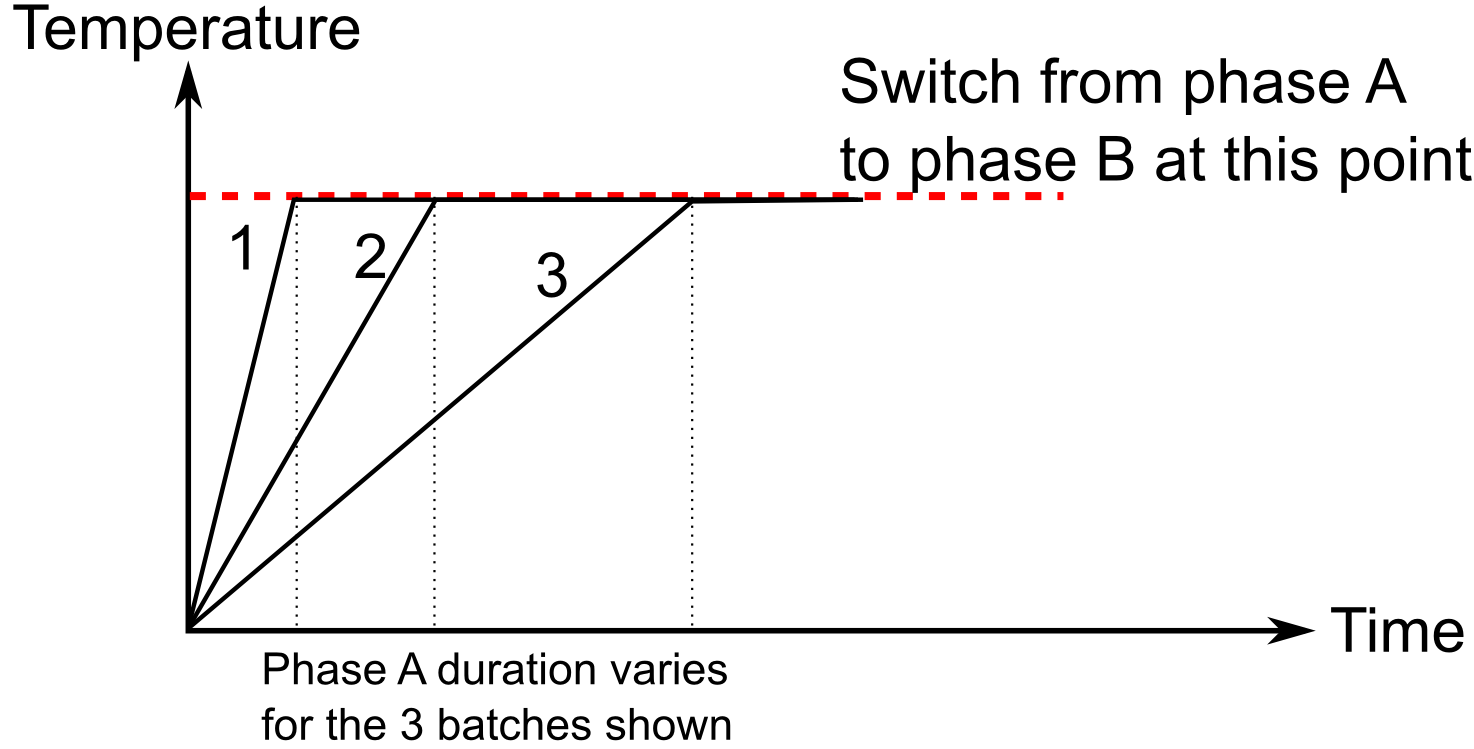
\includegraphics[width=0.7\textwidth]{images/alignment-due-to-phase-switching.png}
					\end{center}

			\item	When operator has wide discretion: causes alignment problems
		\end{itemize}
		\vspace{12pt}
		
	\column{0.3\textwidth}
	
		\begin{center}
			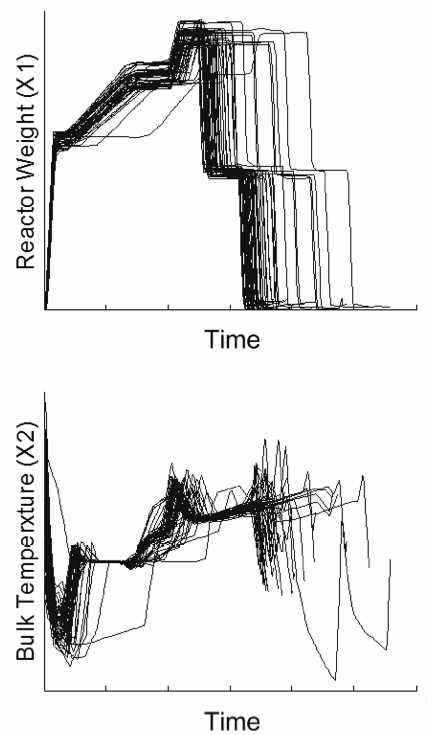
\includegraphics[width=\textwidth]{images/unaligned-trajectories-many-batches.png}
		\end{center}

		\small
		\textbf{Result}: similar trajectories of different duration
\end{columns}
\end{frame}

\begin{frame}\frametitle{Batch alignment: how to align}

Some automated tools are becoming available.  Best results still require case-specific knowledge.
\begin{itemize}
	
	\item	{\color{myGreen}{\emph{Data trimming}}}: throw out data points at start or end of each phase to match average duration.
	
			\begin{itemize}
				\item	\alert{Risk}:  most informative data often near start or end
			\end{itemize}
			
			\pause
	
	\item	{\color{myGreen}{\emph{Dynamic time warping}}}: stretch and shrink data to match a ``golden'' batch
	
			\begin{itemize}
				\item	Hard (impossible?) for real-time monitoring
			\end{itemize}
			
			\pause
	
	\item	{\color{myGreen}{\emph{Indicator variable}}}: find/create a monotonic variable within each phase and apply linear interpolation against it.
		
\end{itemize}

\end{frame}

\begin{frame}\frametitle{Batch alignment: aligning with an indicator}

\begin{itemize}
	
	\item	Good results if indicator is related to batch maturity
	
	\item	Adjust all other variables in phase against this indicator, and interpolate all batches to same number of \( J \) time points
	
	\item	Examples: 
			
			\begin{itemize}
				\item	temperature ramp
				
				\item	amount of raw material fed (semi-batch systems)
				
				\item	create a calculated variable, e.g. the total conversion
				
				\item	lance position in injection molding
			\end{itemize}
			
			\pause
	
	\item	Can be used for online, real-time monitoring (e.g. extrapolate temperature slope, use amount of material fed) \pause
	
	\item	Put the alignment information into \( Z \): very useful for diagnosis
\end{itemize}

\todo{Put some alignment diagrams from Cecilia's thesis here}

\end{frame}

